{\bf \Large
\begin{tabular}{ccc}
\hline
  Corresponding author & : & Hirofumi Tomita\\
\hline
\end{tabular}
}

\section{Spatial descretization}
We employ the Arakawa-C staggered grid with the 3-dimensional momentum
($\rho u, \rho v, \rho w$), density ($\rho$) and mass-weighted potentail temperature($\rho \theta$)
as the prognostic variables.
Figure \ref{fig:cntrl-volume}(a) shows the structure of the control volume for the mass,
indicating the location of each of prognostic variables.
Conceptually, we use the 4th order central difference scheme
for the advection or convection terms and
the 2nd order central difference scheme for the other terms.
Before the descretization of differential equations,
we should diagnose several quantities from the prognostic variables.
\begin{description}
\item[Full-level pressure and potential temperature]
\begin{eqnarray}
&&p_{i,j,k}=p_{00}\left[\frac{(\rho \theta)_{i,j,k} R^*}{p_{00}} \right]^{\frac{c_{p}^*}{c_{p}^*- R^*}}\\
&&\theta_{i,j,k} = \frac{(\rho \theta)_{i,j,k}}{\rho_{i,j,k}} \label{eq:theta full} \\
\end{eqnarray}
\item[Half-level density]
\begin{eqnarray}
&&  \overline{\rho}_{i+\frac{1}{2},j,k} = \frac{\rho_{i+1,j,k}+\rho_{i,j,k}}{2} \label{eq:rho half i} \\
&&  \overline{\rho}_{i,j+\frac{1}{2},k} = \frac{\rho_{i,j+1,k}+\rho_{i,j,k}}{2} \label{eq:rho half j} \\
&&  \overline{\rho}_{i,j,k+\frac{1}{2}} = \frac{\Delta z_k\rho_{i,j,k+1}+\Delta z_{k+1}\rho_{i,j,k}}{\Delta z_k + \Delta z_{k+1}} \label{eq:rho half k}
\end{eqnarray}
\item[Half-level velocity]
\begin{eqnarray}
&&  \overline{u}_{i+\frac{1}{2},j,k} = \frac{(\rho u)_{i+\frac{1}{2},j,k}}{\overline{\rho}_{i+\frac{1}{2},j,k}}\\
&&  \overline{v}_{i,j+\frac{1}{2},k} = \frac{(\rho v)_{i,j+\frac{1}{2},k}}{\overline{\rho}_{i,j+\frac{1}{2},k}}\\
&&  \overline{w}_{i,j,k+\frac{1}{2}} = \frac{(\rho w)_{i,j,k+\frac{1}{2}}}{\overline{\rho}_{i,j,k+\frac{1}{2}}}
\end{eqnarray}
\item[Full-level velocity]
\begin{eqnarray}
&&  \overline{u}_{i,j,k} = \frac{(\rho u)_{i+\frac{1}{2},j,k}+(\rho u)_{i-\frac{1}{2},j,k}}{2\rho_{i,j,k}} \label{eq:u full} \\
&&  \overline{v}_{i,j,k} = \frac{(\rho v)_{i,j+\frac{1}{2},k}+(\rho v)_{i,j-\frac{1}{2},k}}{2\rho_{i,j,k}} \label{eq:v full} \\
&&  \overline{w}_{i,j,k} = \frac{(\rho w)_{i,j,k+\frac{1}{2}}+(\rho w)_{i,j,k-\frac{1}{2}}}{2\rho_{i,j,k}} \label{eq:w full}
\end{eqnarray}
\end{description}




\subsection{Continuity equation}
\begin{eqnarray}
%%
\left(\frac{\partial \rho}{\partial t}\right)_{i,j,k}
&=& - \frac{(\rho u)_{i+\frac{1}{2},j,k} -(\rho u)_{i-\frac{1}{2},j,k}}{\Delta x}\nonumber\\
& & - \frac{(\rho v)_{i,j+\frac{1}{2},k} -(\rho v)_{i,j-\frac{1}{2},k}}{\Delta y}\nonumber\\
& & - \frac{(\rho w)_{i,j,k+\frac{1}{2}} -(\rho w)_{i,j,k-\frac{1}{2}}}{\Delta z}
\end{eqnarray}

\subsection{Momentum equations}
Figure \ref{fig:cntrl-volume}(a) shows the structure of the control volume for the momentum
in the x direction.
The momentum equation is descretized as
\begin{eqnarray}
%%
\left(\frac{\partial \rho u}{\partial t}\right)_{i+\frac{1}{2},j,k}
&=& - \frac{\overline{(\rho u)}_{i+1,j,k} \overline{u}_{i+1,j,k}
           -\overline{(\rho u)}_{i,j,k} \overline{u}_{i,j,k}}
     {\Delta x}\nonumber\\
& & - \frac{\overline{(\rho u)}_{i+\frac{1}{2},j+\frac{1}{2},k}  \overline{v}_{i+\frac{1}{2},j+\frac{1}{2},k}
           -\overline{(\rho u)}_{i+\frac{1}{2},j-\frac{1}{2},k}  \overline{v}_{i+\frac{1}{2},j-\frac{1}{2},k}}
     {\Delta y}\nonumber\\
& & - \frac{\overline{(\rho u)}_{i+\frac{1}{2},j,k+\frac{1}{2}}  \overline{w}_{i+\frac{1}{2},j,k+\frac{1}{2}}
           -\overline{(\rho u)}_{i+\frac{1}{2},j,k-\frac{1}{2}}  \overline{w}_{i+\frac{1}{2},j,k-\frac{1}{2}}}
     {\Delta z}\nonumber\\
& & -\frac{p_{i+1,j,k}-p_{i,j,k}}{\Delta x},
\end{eqnarray}
where
\begin{eqnarray}
&& \overline{(\rho u)}_{i,j,k} \nonumber\\
= && \frac{-(\rho u)_{i+\frac{3}{2},j,k}+7(\rho u)_{i+\frac{1}{2},j,k}+7(\rho u)_{i-\frac{1}{2},j,k}-(\rho u)_{i-\frac{3}{2},j,k}}{12}\\
&& \overline{(\rho u)}_{i+\frac{1}{2},j+\frac{1}{2},k} \nonumber\\
= && \frac{-(\rho u)_{i+\frac{1}{2},j+2,k}+7(\rho u)_{i+\frac{1}{2},j+1,k}+7(\rho u)_{i+\frac{1}{2},j,k}-(\rho u)_{i+\frac{1}{2},j-1,k}}{12}\\
&& \overline{(\rho u)}_{i+\frac{1}{2},j,k+\frac{1}{2}} \nonumber\\
= &&\frac{-(\rho u)_{i+\frac{1}{2},j,k+2}+7(\rho u)_{i+\frac{1}{2},j,k+1}+7(\rho u)_{i+\frac{1}{2},j,k}-(\rho u)_{i+\frac{1}{2},j,k-1}}{12}
\end{eqnarray}
and the velocities at the cell wall for the staggered control volume to $x$ direction are
defined as
\begin{eqnarray}
\overline{u}_{i,j,k} &=& \frac{\overline{u}_{i+\frac{1}{2},j,k}+\overline{u}_{i-\frac{1}{2},j,k}}{2}\\
\overline{v}_{i+\frac{1}{2},j+\frac{1}{2},k} &=&
\frac{\overline{v}_{i,j+\frac{1}{2},k}+\overline{v}_{i+1,j+\frac{1}{2},k}}{2}\\
\overline{w}_{i+\frac{1}{2},j,k+\frac{1}{2}} &=&
\frac{\overline{w}_{i,j,k+\frac{1}{2}}+\overline{w}_{i+1,j,k+\frac{1}{2}}}{2}
\end{eqnarray}
In this form, the 4th order accuracy is guaranteed
on the condition of the constant velocity.

The momentum equations in the $y$ and $z$ directions are descretized
in the same way:
\begin{eqnarray}
%%
\left(\frac{\partial \rho v}{\partial t}\right)_{i,j+\frac{1}{2},k}
&=& - \frac{\overline{(\rho v)}_{i+\frac{1}{2},j+\frac{1}{2},k}  \overline{u}_{i+\frac{1}{2},j+\frac{1}{2},k}
           -\overline{(\rho v)}_{i-\frac{1}{2},j+\frac{1}{2},k}  \overline{u}_{i-\frac{1}{2},j+\frac{1}{2},k}}
     {\Delta x}\nonumber\\
& & - \frac{\overline{(\rho v)}_{i,j+1,k} \overline{v}_{i,j+1,k}
           -\overline{(\rho v)}_{i,j,k} \overline{v}_{i,j,k}}
     {\Delta y}\nonumber\\
& & - \frac{\overline{(\rho v)}_{i,j+\frac{1}{2},k+\frac{1}{2}}  \overline{v}_{i,j+\frac{1}{2},k+\frac{1}{2}}
           -\overline{(\rho v)}_{i,j+\frac{1}{2},k-\frac{1}{2}}  \overline{v}_{i,j+\frac{1}{2},k-\frac{1}{2}}}
     {\Delta z}\nonumber\\
& & -\frac{p_{i,j+1,k}-p_{i,j,k}}{\Delta y},\\
%%
\left(\frac{\partial \rho w}{\partial t}\right)_{i,j,k+\frac{1}{2}}
&=& - \frac{\overline{(\rho w)}_{i+\frac{1}{2},j,k+\frac{1}{2}}  \overline{u}_{i+\frac{1}{2},j,k+\frac{1}{2}}
           -\overline{(\rho w)}_{i-\frac{1}{2},j,k+\frac{1}{2}}  \overline{u}_{i-\frac{1}{2},j,k+\frac{1}{2}}}
     {\Delta x}\nonumber\\
& & - \frac{\overline{(\rho w)}_{i,j+\frac{1}{2},k+\frac{1}{2}}  \overline{w}_{i,j+\frac{1}{2},k+\frac{1}{2}}
           -\overline{(\rho w)}_{i,j-\frac{1}{2},k+\frac{1}{2}}  \overline{w}_{i,j-\frac{1}{2},k+\frac{1}{2}}}
     {\Delta y}\nonumber\\
& & - \frac{\overline{(\rho w)}_{i,j,k+1} \overline{w}_{i,j,k+1}
           -\overline{(\rho w)}_{i,j,k} \overline{w}_{i,j,k}}
     {\Delta z}\nonumber\\
& & -\frac{p_{i,j,k+1}-p_{i,j,k}}{\Delta z}-\overline{\rho}_{i,j,k+\frac{1}{2}} g
\end{eqnarray}

\subsubsection{Pressure}
Since the pressure pertubation is much smaller than the absolute value of the pressure,
truncation error of floating point value is relatively large and its precision could become smaller.
Therefore, the pressure gradient terms are calculated from the deviation from reference pressure field satisfing the hydrostatic balance.
Additionally, the calculation of the pressure (eq. \ref{eq: pressure}) is linearlized avoiding a power calculation, which numerically costs expensive.
\begin{align}
% p = p_{00}\left(\frac{\rho \theta R^*}{p_{00}} \right)^{\frac{c_{p}^*}{c_{p}^*- R^*}}
  p
  &\approx \bar{p} + \frac{c_p^*}{R^* C_v^*}\left(\frac{\rho \theta R^*}{p_{00}}\right)^{\frac{R^*}{c_{v}^*}}  \{\rho \theta - \overline{\rho \theta}\} \nonumber \\
  &= \bar{p} + \frac{c_p^*}{c_v^*} \frac{\bar{p}}{\overline{\rho \theta}} (\rho \theta)' \\
  p &- p_\mathrm{ref}
  = \bar{p} - p_\mathrm{ref}
  + \frac{c_p^*}{c_v^*} \frac{\bar{p}}{\overline{\rho \theta}} (\rho \theta)'
\end{align}


\subsection{Energy equation}

\begin{eqnarray}
%%
\left(\frac{\partial \rho \theta}{\partial t}\right)_{i,j,k}
&=& - \frac{(\rho u)_{i+\frac{1}{2},j,k} \overline{\theta}_{i+\frac{1}{2},j,k}
           -(\rho u)_{i-\frac{1}{2},j,k} \overline{\theta}_{i-\frac{1}{2},j,k}}
     {\Delta x}\nonumber\\
& &  - \frac{(\rho v)_{i,j+\frac{1}{2},k} \overline{\theta}_{i,j+\frac{1}{2},k}
           -(\rho v)_{i,j-\frac{1}{2},k} \overline{\theta}_{i,j-\frac{1}{2},k}}
     {\Delta y}\nonumber\\
& &  - \frac{(\rho w)_{i,j,k+\frac{1}{2}} \overline{\theta}_{i,j,k+\frac{1}{2}}
           -(\rho w)_{i,j,k-\frac{1}{2}} \overline{\theta}_{i,j,k-\frac{1}{2}}}
     {\Delta z}\nonumber\\
\end{eqnarray}
where
\begin{eqnarray}
&& \overline{\theta}_{i+\frac{1}{2},j,k} =
\frac{-\theta_{i+2,j,k}+7\theta_{i+1,j,k}+7\theta_{i,j,k}-\theta_{i-1,j,k}}{12}\\
&& \overline{\theta}_{i,j+\frac{1}{2},k} =
\frac{-\theta_{i,j+2,k}+7\theta_{i,j+1,k}+7\theta_{i,j,k}-\theta_{i,j-1,k}}{12}\\
&& \overline{\theta}_{i,j,k+\frac{1}{2}} =
\frac{-\theta_{i,j,k+2}+7\theta_{i,j,k+1}+7\theta_{i,j,k}-\theta_{i,j,k-1}}{12}
\end{eqnarray}

\subsection{Tracer advection}
The tracer advection process is done after the time integration of
the dynamical variables ($\rho$, $\rho u,\rho v,\rho w$, and $\rho \theta$).
We impose two constraints to tracer advection:
\begin{description}
\item[Consistency With Continuity ( CWC )]
On the condition without any source/sink,
the mass concentration in the advection process
should be conserved along the trajectory.
It is, at least, necessary that
the spatially constant mass concentration should be kept
in any motion of fluid.
In order to satisfy this condition, we use the same mass flux at the last Runge-Kutta
process of Eqs.() and () for integration of tracers:
\begin{eqnarray}
%%
\frac{\left(\rho q\right)^{n+1}_{i,j,k} - \left(\rho q\right)^{n}_{i,j,k}}{\Delta t}
&=& - \frac{(\rho u)_{i+\frac{1}{2},j,k} \overline{q}_{i+\frac{1}{2},j,k}
           -(\rho u)_{i-\frac{1}{2},j,k} \overline{q}_{i-\frac{1}{2},j,k}}
     {\Delta x}\nonumber\\
& &  - \frac{(\rho v)_{i,j+\frac{1}{2},k} \overline{q}_{i,j+\frac{1}{2},k}
           -(\rho v)_{i,j-\frac{1}{2},k} \overline{q}_{i,j-\frac{1}{2},k}}
     {\Delta y}\nonumber\\
& &  - \frac{(\rho w)_{i,j,k+\frac{1}{2}} \overline{q}_{i,j,k+\frac{1}{2}}
           -(\rho w)_{i,j,k-\frac{1}{2}} \overline{q}_{i,j,k-\frac{1}{2}}}
     {\Delta z}\nonumber\\
\label{eq:tracer_int}
\end{eqnarray}
\item[Monotonicity]
In order to satisfy the monotonicity of tracer advection,
we employ the Flux Corrected Trasport scheme, which is a hybrid scheme
with the 4th order central difference scheme and 1st order upwind scheme.
If The 4th order central difference is applied,
$\overline{q}$ is descritized as
\begin{eqnarray}
&& \overline{q}_{i+\frac{1}{2},j,k}^{high} =
\frac{-q_{i+2,j,k}+7q_{i+1,j,k}+7q_{i,j,k}-q_{i-1,j,k}}{12}\\
&& \overline{q}_{i,j+\frac{1}{2},k}^{high} =
\frac{-q_{i,j+2,k}+7q_{i,j+1,k}+7q_{i,j,k}-q_{i,j-1,k}}{12}\\
&& \overline{q}_{i,j,k+\frac{1}{2}}^{high} =
\frac{-q_{i,j,k+2}+7q_{i,j,k+1}+7q_{i,j,k}-q_{i,j,k-1}}{12}.
\end{eqnarray}
On the other hand, in the 1st order upwind scheme 
$\overline{q}$ is described as
\begin{eqnarray}
\overline{q}_{i+\frac{1}{2},j,k}^{low} =
\begin{cases}
  q_{i,j,k} & ( (\rho u)_{i+\frac{1}{2},j,k}>0 )\\
  q_{i+1,j,k} & ({\rm otherwise})\\
\end{cases}
\\
\overline{q}_{i,j+\frac{1}{2},k}^{low} =
\begin{cases}
  q_{i,j,k} & ( (\rho u)_{i,j+\frac{1}{2},k}>0 )\\
  q_{i,j+1,k} & ({\rm otherwise})\\
\end{cases}
\\
\overline{q}_{i,j,k+\frac{1}{2}}^{low} =
\begin{cases}
  q_{i,j,k} & ( (\rho u)_{i,j,k+\frac{1}{2}}>0 )\\
  q_{i,j,k+1} & ({\rm otherwise})\\
\end{cases}
\end{eqnarray}
The actual $\overline{q}$ is described as
\begin{eqnarray}
  \overline{q}_{i+\frac{1}{2},j,k}
&=& C_{i+\frac{1}{2},j,k} \overline{q}_{i+\frac{1}{2},j,k}^{high}
+ \left( 1 - C_{i+\frac{1}{2},j,k}\right) \overline{q}_{i+\frac{1}{2},j,k}^{low}\\
  \overline{q}_{i,j+\frac{1}{2},k}
&=& C_{i,j+\frac{1}{2},k} \overline{q}_{i,j+\frac{1}{2},k}^{high}
+ \left( 1 - C_{i,j+\frac{1}{2},k}\right) \overline{q}_{i,j+\frac{1}{2},k}^{low}\\
  \overline{q}_{i,j,k+\frac{1}{2}}
&=& C_{i,j,k+\frac{1}{2}} \overline{q}_{i,j,k+\frac{1}{2}}^{high}
+ \left( 1 - C_{i,j,k+\frac{1}{2}}\right) \overline{q}_{i,j,k+\frac{1}{2}}^{low}
\end{eqnarray}
See the appedix for the method to determine the flux limter.
\end{description}



\section{boundary condition}
The boundary condition only for the vertical velocity at the top and bottom
boundaries is needed:
\begin{eqnarray}
&&  w_{i,j,k_{max}+\frac{1}{2}} = 0\\
&&  w_{i,j,k_{min}-\frac{1}{2}} = 0
\end{eqnarray}
This leads to the boundary condition of the prognostic variable as
\begin{eqnarray}
&&  (\rho w)_{i,j,k_{max}+\frac{1}{2}} = 0\\
&&  (\rho w)_{i,j,k_{min}-\frac{1}{2}} = 0
\end{eqnarray}



\section{Numerical filters}
We impose an explicit numerical filter using the numerical viscosity and diffusion.
Although the filter is necessary for numerical stability, too strong a~filter could dampen any physically meaningful variability.
In this subsection, we describe the numerical filters used in this model, and discuss the strength of the filter.


In order to damp the higher wavenumber component selectively, we adopt the hyperviscosity and diffusion in the traditional way.
The hyperviscosity and diffusion of the $n$th order is defined as
\begin{align}
&\frac{\partial }{\partial x}\left[\nu \rho \frac{\partial^{n-1} f}{\partial x^{n-1}}\right], \label{eq:num-diff-def}
\end{align}
where $f$ is an arbitrary variable $(f \in \rho, u, v, w, \theta, q)$.

The Laplacian of $f$ is discretized as
\begin{align}
&\Delta f_i = \frac{1}{\Delta x_i}
\left[
 \frac{1}{\Delta x_{i+\frac{1}{2}}}f_{i+1}
-\left(\frac{1}{\Delta x_{i+\frac{1}{2}}}+\frac{1}{\Delta x_{i-\frac{1}{2}}}\right)f_i
 +\frac{1}{\Delta x_{i-\frac{1}{2}}}f_{i-1}\right],
\end{align}
and
\begin{align}
\Delta^{n/2} f_i =~&\frac{1}{\Delta x_i}
\left[
 \frac{1}{\Delta x_{i+\frac{1}{2}}}\Delta^{n/2-1}f_{i+1}
-\left(\frac{1}{\Delta x_{i+\frac{1}{2}}}+\frac{1}{\Delta x_{i-\frac{1}{2}}}\right)\Delta^{n/2-1}f_i
 \right.\nonumber\\&\left.\,\,+\frac{1}{\Delta x_{i-\frac{1}{2}}}\Delta^{n/2-1}f_{i-1}\right].
   \end{align}
   Here we consider spatially dependent grid interval in calculating
   the Laplacian.  If it is calculated with constant $\Delta x_i$ as
\begin{align}
&\Delta f_i =
  \frac{1}{\Delta x_i^2} \left(f_{i+1} -2f_i +f_{i-1}\right), \\
&  \Delta^{n/2} f_i =
  \frac{1}{\Delta x_i^2} \left(\Delta^{n/2-1}f_{i+1} -2\Delta^{n/2-1}f_i +\Delta^{n/2-1}f_{i-1}\right),
\end{align}
non-negligible numerical noise appears where the grid spacing varies (e.g.,  stretching layer near the top boundary).

The hyperviscosity and diffusion can be discretized as
\begin{align}
&\frac{\partial }{\partial x}\left[\nu \rho \frac{\partial^{n-1} f}{\partial^{n-1} x}\right] \sim
\frac{F_{i+\frac{1}{2}}-F_{i-\frac{1}{2}}}{\Delta x_{i}},
\label{eq:num-diff}
\end{align}
where
\begin{align}
&F_{i+\frac{1}{2}}  \frac{\nu_{i+\frac{1}{2}}\rho_{i+\frac{1}{2}}}{\Delta x_{i+\frac{1}{2}}}
       \left( \Delta^{n/2-1} f_{i+1} - \Delta^{n/2-1} f_i \right).
\label{eq:num-diff-F}
\end{align}

The coefficient, $\nu$, is written as
\begin{align}
&\nu_{i+\frac{1}{2}} = (-1)^{n/2+1} \gamma \frac{\Delta x_{i+\frac{1}{2}}^n}{2^n\Delta t},
\end{align}
where $\gamma$ is a~non-dimensional coefficient.
One-dimensional sinusoidal two-grid noise will decay to $1/e$ with $1/\gamma$ time steps.
Note that the theoretical e-folding time is $\frac{2^n}{\pi^n}\frac{\Delta t}{\gamma}$.
However, it is $\frac{\Delta t}{\gamma}$ with the fourth-order central scheme used in this model.


For the numerical stability of the numerical filter itself, it should satisfy
\begin{align}
&\gamma < 1
\end{align}
for the one-dimensional two-grid noise, and
\begin{align}
&\gamma < \frac{1}{3} \label{eq:condition-gamma}
\end{align}
for the three-dimensional two-grid noise.
The conditions might be stricter for other types of noise.

The flux, $F$, for the numerical filter is added to the advective flux as
\begin{align}
&(\rho u f)_{i+\frac{1}{2}}^{\dagger} = (\rho u f)_{i+\frac{1}{2}}+F_{i+\frac{1}{2}},
\end{align}
where the first term of the right-hand side is the flux calculated by the advection scheme.
In the present model, the advection scheme is the fourth-order central difference scheme.
This concept is very important for the CWC condition in the tracer equations.
The modified mass flux of the numerical filter should be used in the tracer advection, otherwise the CWC condition is violated.

The numerical viscosity and diffusion in the $y$ and $z$ directions are formulated in the same way as in the $x$~direction, although a~special treatment for the $z$ direction is needed.
At the top and bottom boundaries, the flux must be zero, $F_{k_{\max}+\frac{1}{2}} = F_{k_{\min}-\frac{1}{2}} = 0$.
In order to calculate the $F_{k_{\max}-\frac{1}{2}}$ and $F_{k_{\min}+\frac{1}{2}}$, values beyond the boundaries, $f_{k_{\max}+1}$ and $f_{k_{\min}-1}$, are required, then the mirror boundary condition is assumed; $f_{k_{\max}+1} = -f_{k_{\max}}$ and $f_{k_{\min}-1} = -f_{k_{\min}}$.
This condition is appropriate to cause the decay the vertical two-grid noise.


Vertical profiles of density, potential temperature, and water vapor usually have significant (e.g., logarithmic) dependencies on height.
Eq.~(\ref{eq:num-diff}) has a~non-zero value even for the steady state, and the numerical filter produces artificial motion.
To reduce this artificial motion, we introduce a~reference profile which is a~function of height, and deviation from the reference is used as $f$ instead of $\rho$, $\theta$, and $q_{\mathrm{v}}$ in calculating the numerical filter.
The reference profile can be chosen arbitrarily, but a~profile under hydrostatic balance is usually chosen.





\begin{figure}[t]
\begin{center}
  \begin{tabular}{l}
    (a) Control volume for the mass\\
  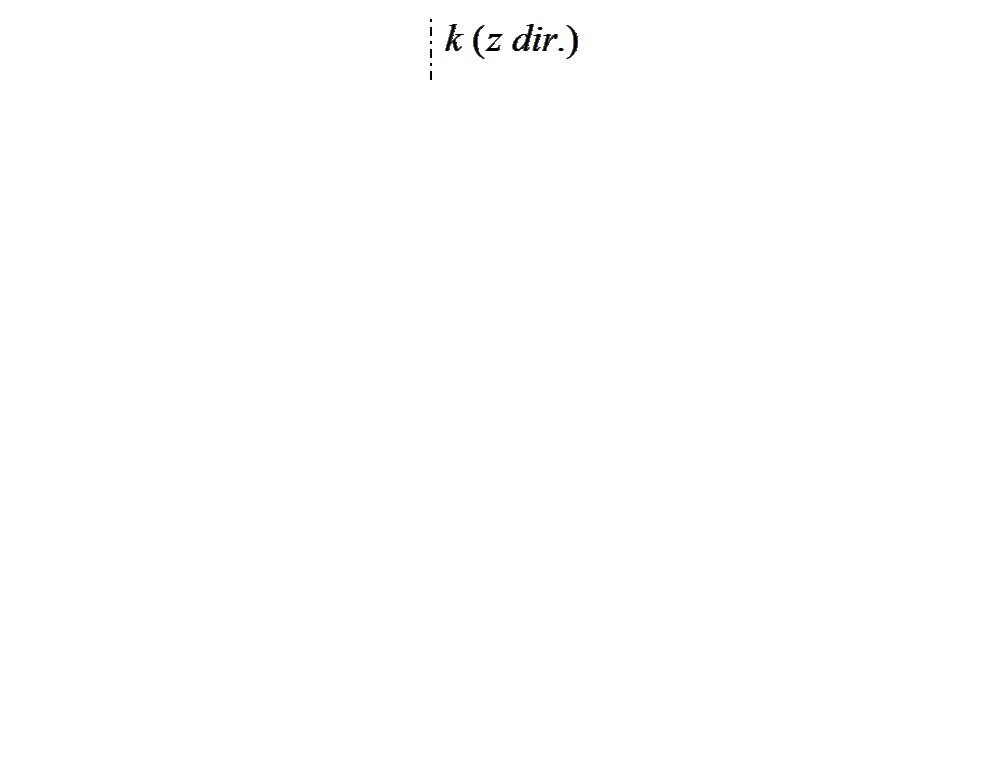
\includegraphics[scale=0.6]{./../figure/cntrl-volume.eps}\\
    (b) Control volume for the momentum\\
  \includegraphics[scale=0.6]{./../figure/cntrl-volume2.eps}\\
  \end{tabular}
\end{center}
  \caption{Control volume}
  \label{fig:cntrl-volume}
\end{figure}
